\chapter{Beszélőazonosító rendszerek napjainkban}

\section{Beszéd adathalmazok}

\section{TIMIT}

\section{CMU Arctic}

\section{WaveNet classifier}

\subsection{WaveNet}

A WaveNet egy mély neurális hálózat audio hullámformák generálásához, amelyet a Google DeepMind publikált 2016-ban. Az ötletet az akkori felfedezések adták neurális autoregresszív generatív modellezés terén, amelyeket komplex eloszlások, például képek modellezésére használtak (van den Oord et al., 2016a;b). Ezt felhasználva audio hullámformák generálásában új eredményeket értek el.

\begin{itemize}
	\item Képes olyan természetes hangzású beszéd hullámformák generálására, amit korábban parametrikus vagy konkatenatív beszédszintézissel sosem értek el. 
	\item Az audio hullámformák generáláshoz szükséges nagy receptív mezőt hatékonyan, nyújtott kauzális konvolúciókkal implementálja.
	\item Ha a modellt a beszélők identitásával tanítják, képes új hangok generálására.
	\item A zene generálás és a beszédfelismerés terén is ígéretesnek bizonyult.
\end{itemize}

\subsubsection{Nyújtott kauzális konvolúció}

A modell autoregresszív, vagyis a kimenete korábbi időpillanatokban felvett értékeitől függ. Ez azért fontos, mert a WaveNet egy generatív modell. A generált hullámforma \emph{t}-edik időpillanatbeli értéke nem függhet jövőbeli értékektől. A kauzalitás legegyszerűbb implementációja ha legalább a \emph{kernel-1} méretű paddinget adunk a konvolúcióhoz.

\begin{figure}[!ht]
	\centering
	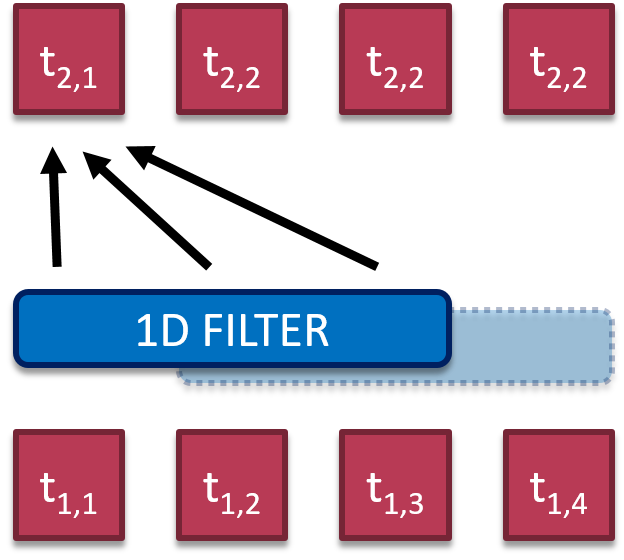
\includegraphics[width=80mm, keepaspectratio]{figures/1d-conv.png}
	\caption{1D nem kauzális konvolúció.}
	\label{fig:1d_noncausal_conv}
\end{figure}

\begin{figure}[!ht]
	\centering
	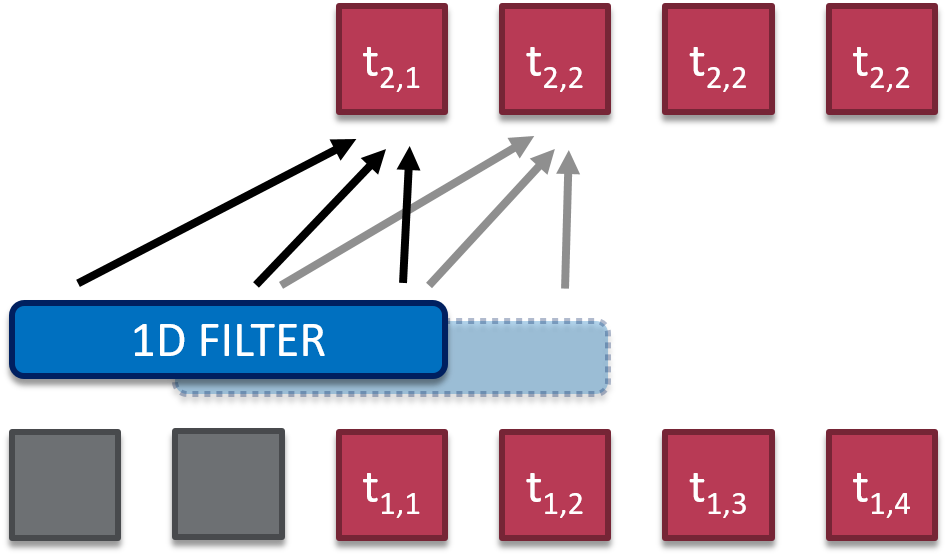
\includegraphics[width=120mm, keepaspectratio]{figures/1d-causal-conv.png}
	\caption{1D kauzális konvolúció paddinggel.}
	\label{fig:1d_causal_conv}
\end{figure}

\newpage

A \ref{fig:1d_noncausal_conv} ábra egy nem kauzális 1D konvolúciót mutat. A $t_{i, j}$ az i-edik rétegbeli j-edik neuron. Látható, hogy a $t_{2,1}$ jövőbeli időpillanatokból kap értékeket a szűrőn keresztül. Ennek megoldása a szűrő eltolása padding segítségéve. Ezt szemlélteti a \ref{fig:1d-causal-conv} ábra, ahol az egyes neuronok csak korábbi időpillanatokból kapnak értékeket. 

A beszéd generálásánál a \emph{t}-edik időpillanatban a hullámforma értéke a korábbi adatoktól függ. Ahhoz, hogy magas frekvenciájú, pl. 16 kHz frekvencián mintavételezett 
hangadattal tanítsuk a hálózatot nagy receptív mezőre van szükség. A receptív mező az a szélesség, amit a szűrő lát a bemenetből. 16 kHz esetén egy másodpercnyi jelet 16000 szám reprezentál. Ahhoz, hogy a hálózat helyesen jósolja meg a következő generált értéket, a hosszú távú dependenciákat figyelembe kell vennie, tehát a receptív mező méretét elég nagyra kell megválasztani. A probléma ekkora mezők esetén, hogy sok konvolúciós réteget igényelnek (egy korábbi időpillanatbeli adat plusz egy konvolúciós réteget igényel), ami növeli a számítási komplexitást. A nyújtott konvolúciók erre adnak hatékony megoldást. A filter meghatározott távolságokkal kihagy valamennyi inputot, majd figyelembe vesz egyet. Egymás utáni rétegekben a nyújtási tényezőt exponenciálisan növelve a receptív mező is exponenciálisan fog nőni.

\begin{figure}[!ht]
	\centering
	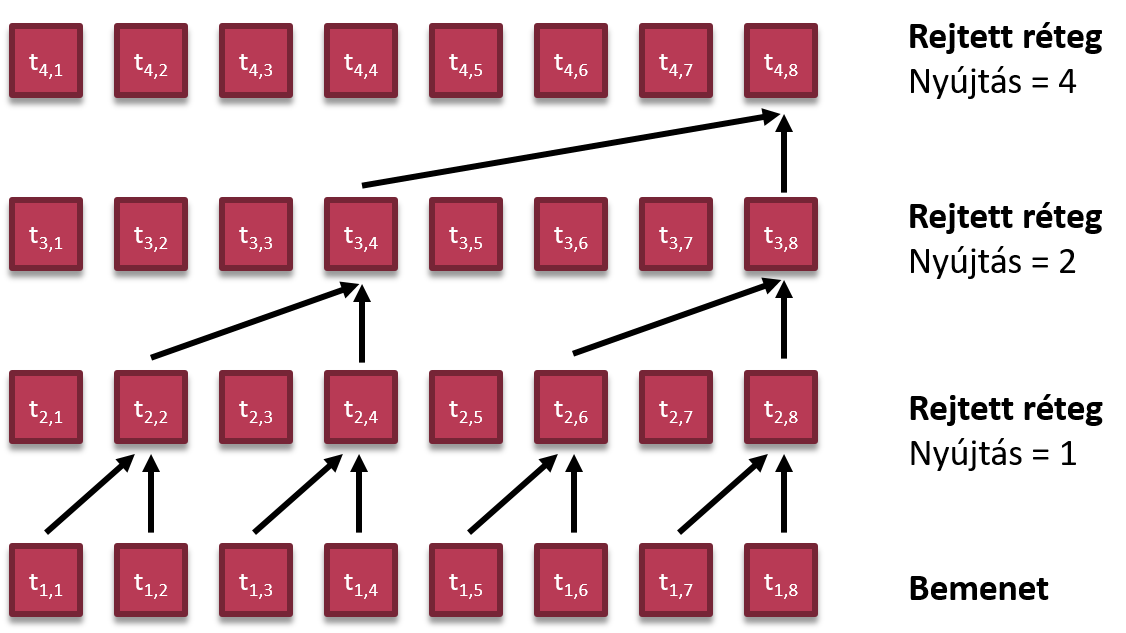
\includegraphics[width=150mm, keepaspectratio]{figures/1d-dilated-conv.png}
	\caption{1D nyújtott kauzális konvolúciós rétegek.}
	\label{fig:1d_dilated_conv}
\end{figure}

\subsubsection{SoftMax eloszlás}
A WaveNet SoftMax réteget használ a $p(x_t|x_1,\dots,x_t)$ feltételes valószínűségi eloszlás modellezésére.
Az audio jeleket általában 16 bites egészekkel kódolják, amelyek 65536 értéket vehetnek fel. Ebben az esetben a SoftMax rétegnek 65536 valószínűséget kell kimenetként adnia, melyek összege 1. A $\mu$-law kvantálást alkalmazva a beszédjel 256 biten kódolható és később az inverz transzformációval jó minőségben visszaállítható.

Az emberi hallás sokkal érzékenyebb alacsony amplitúdójú hangok kvantálási zajára, mint a magasabbakéra. Erre alapozva a $mu$-law kvantáló a jelet egy logaritmikus függvénnyel kvantálja úgy, hogy az alacsonyabb amplitúdójú jelek nagyobb felbontással (több bittel), a magasabbak pedig kisebbel lesznek kódolva. Ez növeli a SoftMax réteg hatékonyságát is, mert nagyobbak lesznek a valószínűségek közötti különbségek.

A tanítást a WaveNet klasszifikációs problémaként kezeli. A bemeneteket OneHot kódolással adjuk meg, a SoftMax réteg pedig az így kódolt egészekre ad valószínűségi eloszlást.

\subsubsection{Reziduális blokkok}

A WaveNet architektúra egymáshoz csatolt reziduális blokkokból és ún. kapcsolat-ugrásokból (skip-connection) épül föl. A reziduális hálózatok előnye, hogy orvosolják az elenyésző gradiens problémát, így sokkal mélyebb hálózat építhető.

\begin{figure}[!ht]
	\centering
	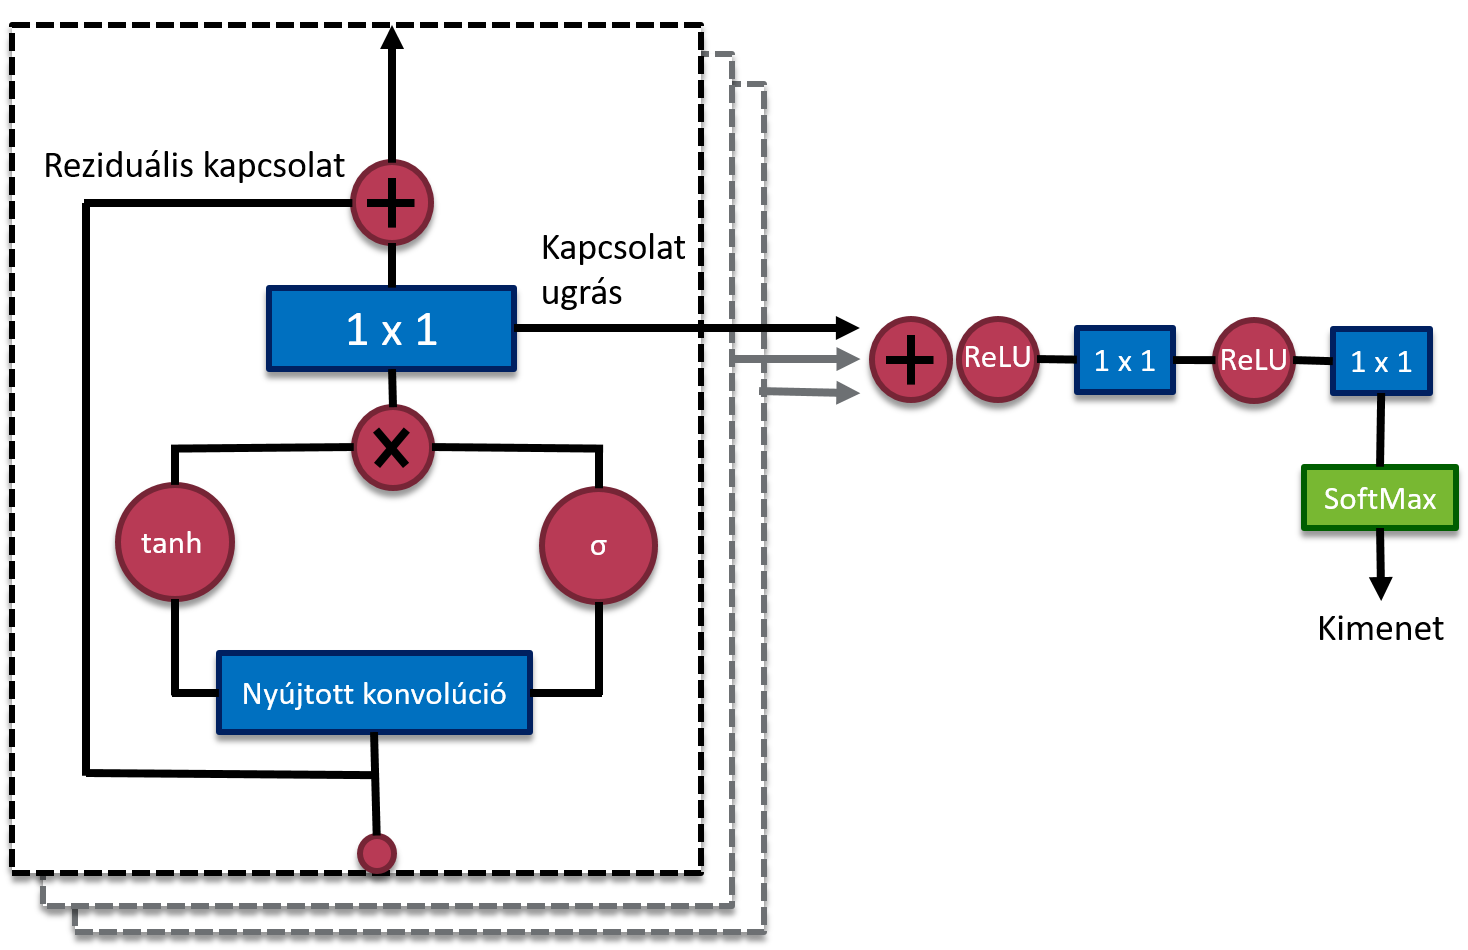
\includegraphics[width=150mm, keepaspectratio]{figures/wavenet_arch.png}
	\caption{WaveNet architektúra.}
	\label{fig:wavenet_arch}
\end{figure}

Egy reziduális blokk bemenete egy 2x1-es konvolúciós rétegen megy keresztül. Balra egy \emph{tanh}, jobbra egy szigmoid aktivációs függvényen haladnak át, majd elemenkénti szorzás és 1x1 konvolúció után egyrészt átugorja a reziduális kapcsolatot, illetve azzal együtt bemenetként szolgál a következő reziduális egységnek. Az 1x1 konvolúciós rétegek a dimenzionalitás változtatására szolgál. Külön 1x1 konvolúciós szűrők skálázzák a kimenetet a következő reziduális blokk bemenetére, és a kapcsolat-ugrásokhoz.

\subsection{Módosított WaveNet architektúra}

\subsection{Eredmények}

\section{SincNet}

\subsection{Eredmények}